\section{Nonlinear finite element method} \label{sec:C1:fem}
In this section, we will introduce the preliminaries for the nonlinear topology optimization method by briefly discussing the nonlinear FEM. The approach is similar to FEM but it accounts for various nonlinear aspects in continuum mechanics. It is particularly useful for modeling large geometrical deformations and hyper-elasticity, which cannot be accurately represented using linear FEM variants. These descriptions are essential in understanding how soft materials deform, and therefore can be beneficial to explore in optimal design solutions for soft materials.

\subsection{Strain theory in continuum mechanics}
We start by presenting the variational principle of continuum mechanics in a nonlinear geometrical context. Consider an undeformed material domain as $\mathcal{B}_0 \subset \R^3$. When external forces act on $\mathcal{B}_0$, it undergoes both rigid-body and elastic deformation, resulting in a new body, denoted by $\mathcal{B} \subset \R^3$. Let $\XB \in \mathcal{B}_0$ represent an arbitrary material point within the undeformed configuration, whose motion can be described by a continuous path between two position vectors $\XB$ and $\XB'$. These vectors correspond to a particular material point in the undeformed and quasi-static deformed configurations (\ie, zero-velocity), respectively. Suppose that the deformation mapping is described by a flow $\boldsymbol{\varphi}^{(t)}: \mathcal{B}_0 \to \mathcal{B}$ such that $\boldsymbol{X} \mapsto \boldsymbol{\varphi}^{(T)}(\boldsymbol{X}) = \boldsymbol{X}'$ for a time instance $T > 0$ when static equilibrium between elastic deformation and external forces is reached. More conveniently, we can write $\boldsymbol{X}' = \boldsymbol{X} + \dB(\boldsymbol{X},T)$ where $\dB(\XB,T)$ represents the displacement field at the equilibrium configuration.

In the field of continuum mechanics, the primary objective is to determine an approximation of the displacement field $\dB(\XB,T)$ that satisfies the boundary conditions imposed on the initial body $\mathcal{B}$. To achieve this goal, it is necessary to establish a relationship between the displacement and strain, as well as between these strains and the internal stresses caused by elastic deformation. A fundamental measure of deformation is the deformation gradient tensor, which can be computed as follows: assuming that the mapping $\boldsymbol{\varphi}$ is sufficiently smooth \cite{Kim2018,Holzapfel2002}, the second-order deformation gradient tensor is obtained through spatial differentiation:
%
\begin{align}
\boldsymbol{F} := \frac{\p \boldsymbol{\varphi} }{\p \boldsymbol{X}}   = \boldsymbol{I} + \frac{\p \dB }{\p \boldsymbol{X}}.
\label{eq:C2:Fgrad}
\end{align}
%
The deformation gradient tensor, as shown in \eqref{eq:C2:Fgrad}, provides valuable information about the local deformation. Specifically, it describes the deformation of an infinitesimal sub-volume of the material domain $\mathcal{B}_0$ around $\XB$. The volume change of this sub-volume can be calculated using $J := \det{\FB} > 0$. Following convention \cite{Kim2018,Holzapfel2002}, we can derive the Green-Lagrange strain tensor from equation \eqref{eq:C2:Fgrad} as $\ET : = \frac{1}{2}(\FB^\top \FB - \boldsymbol{I})$. In terms of the displacement gradient $\nabla_{0} \dB := \tfrac{\p \dB}{\p \XB}$, the general expression for the Green-Lagrange strain tensor is given by:
%
\begin{align}
\ten{E} & := \frac{1}{2}\big( \nabla_0 \dB  +\nabla_0^\top \dB  + \nabla_0 \dB^\top \, \nabla_0 \dB \big)
\label{eq:E_tens}
\end{align}
%
which is a symmetric second-order tensor. In the context of continuum mechanics, it is crucial to consider the geometric nonlinearities that arise when large deformations occur. Specifically, the term $\nabla_0 \dB^\top \nabla_0 \dB$ captures these nonlinearities. However, most structural optimization methods assume small deformations, \ie, $\nabla_0 \dB^\top \nabla_0 \dB \ll \nabla_0 \dB$, and simplify the strain tensor as $\vec{\varepsilon} = \tfrac{1}{2}\big( \nabla_0 \dB + \nabla_0^\top \dB \big)$, which neglects the last term. Although this is hugely beneficial for numerical performance, this simplification is not always appropriate for soft robotics, where accurate mechanical descriptions require accounting for geometric nonlinearities.

% Since the numerical implementation generally involves matrix-vector notation instead of tensor notation, we briefly introduce the following notation. A Cartesian tensor can be formally represented by an component array in terms of a basis $\eB_i$. For example, a second-order tensor can be denoted by $\TT = \sum_{ij}\TT_{ij}\, \eB_i \otimes \eB_j$ with $\otimes$ the dyadic product and bases $\eB_1,\eB_2,\eB_3 \in \R^3$. As such, the column vector representation of a second-order tensor $\TT$ can be denoted by $\{ \TT \} := \text{vec}({\TT}_{ij})$. Hence, the variational form of Lagrangian strain can be written in vector notation as
% \begin{align}
% \{\delta \boldsymbol{E} \} & = \frac{\p}{\p \varepsilon}\left[\frac{\p \boldsymbol{E}(\x + \varepsilon \cdot \delta \x)}{\p \x} \right]_{\varepsilon = 0} \\ & := \boldsymbol{B}(\boldsymbol{x}) \, \{\delta  \boldsymbol{x}\},
% \end{align}
% where $\boldsymbol{B}(\boldsymbol{x})$ is a nonlinear strain-displacement matrix that relates displacements to Lagrangian strain \cite{Kim2018}. \\ 

% \begin{rmk}[Two-dimensional problems]
% In this work, we primarily focus on two-dimensional mechanical problems. We would like to stress that the variational principle for three-dimensional continuum solids discussed earlier are similar to those in two-dimensional situations \cite{Kim2018,Gain2013}. 
% \end{rmk}

\subsection{Isotropic hyperelasticity materials}
Soft robotics is a field that relies heavily on the use of elastomer materials. These materials possess several desirable properties, such as relatively low Young's moduli, large reversible strains, and mechanical robustness. In material mechanics, these elastic materials are often classified as hyperelastic materials due to their ability to undergo large deformations. As a result of this deformation, rubber-like materials exhibit state-dependent mechanical compliance. Unlike Hookean materials, which have linear elasticity, the constitutive behavior of hyperelastic materials is described by a strain energy density function ${\Psi}: \ten{E} \mapsto \Rp$. This function represents the conservative elastic energy density stored inside the continuum. Therefore, the elastic potential energy is the integration of the energy density over the undeformed domain and can be expressed as:
%
\begin{equation}
\Uf_{\textrm{int}}(\ten{E}):= \int_{\mathcal{B}_0} \Psi(\ten{E})\; dV \ge 0
\end{equation}
%
In literature, $\Psi$ is often chosen as polynomial regression model which fits empirical data of materials, leaving the choice on $\Psi$ generally free. Nevertheless, there exist popular options that are commonly used for rubber-like engineering materials. Popular constitutive models for hyperelastic behavior include Neo-Hookean \cite{Smith2018,Bern2019,Bern2021Apr}, Mooney \cite{Kim2018}, Ogden \cite{Xavier2022Jun}, or Yeoh \cite{Renaud2011}. In contrast to linear elasticity strain energy, the strain energy for hyperelastic constitutive models is commonly expressed in terms of the strain invariants (${I}_1$, ${I}_2$, ${I}_3$).

In this work, a compressible Yeoh constitutive model for hyperelasticity is used to describe the mechanics of soft materials. Let $I_1 = \textrm{tr}(\ten{C})$ be the first strain invariant with $\ten{C} = \mat{F}^\top \mat{F}$ the right Cauchy strain tensor. Then, following the work of Renaud et al. \cite{Renaud2011} and Kim  et al. \cite{Kim2018}, the strain energy function of the compressible Yeoh model is given by:
%
\begin{equation}
{\Psi} = \sum_{i = 1}^{3} c_i (J_1 - 3)^i + \sum_{j = 1}^{3} \frac{1}{d_j} (J - 1)^{2j},
\label{eq:C3:psi_model_yeoh}
\end{equation}
%
where $J_1 = J^{-\tfrac{1}{3}} I_1$ is a modified first strain variant, and $c_1 > 0$ and $c_2$, $c_3$ are the material constants related to stiffness (\si{\newton \per \square \meter}), and the constants $d_{1,2,3} > 0$ related to material compressibility. %The Yeoh model has the potential to considerably decrease the requirement for extensive material testing. As the model depends solely on $J_1$, the material parameters can be obtained solely from a uniaxial tension tests \cite{Renaud2011}. 
%To relate strains to stress given the model \eqref{eq:C3:psi_model_yeoh}, we require the Piolla stress measure. The second Piola- stress of a constitutive material can be calculated by differentiating the strain energy function with respect to the Lagrangian strain tensor \cite{Renaud2011,Kim2018}:

% \begin{equation}
% \ST := \frac{\p {\Psi}}{\p \boldsymbol{E}} = \FB^{-1} \frac{\p \Psi}{\p \FB}%2\frac{\p {\Psi}}{\p \boldsymbol{C}}, 
% \label{eq:piola}
% \end{equation}
% %
% which is a symmetric second-order tensor that is the energy conjugate to the Lagrangian strain. 

\subsection{Variational principle of energy minimization}
A common way of finding solutions to the displacements $\dB$ of continuum solids, is by the variational principle of energy minimization. The method explores the idea that at the equilibrium configuration, the total potential energy of the system has zero variation, \ie, the slope is zero. To explain the method, we follow the work of Kim et al. \cite{Kim2018}. The potential energy of an elastic system is the difference between the internally stored elastic energy $\Uf_{\textrm{int}}$ and the work done by the external forces $\Uf_{\textrm{ext}}$. This work is equivalent by the volume integral of the forces multiplied by their traveled distance, \ie, the displacement field $\dB(\XB,T)$. Thus, using \eqref{eq:C3:psi_model_yeoh}, the total potential energy of the elastic system is
%
\begin{align}
\Uf(\dB) &= \Uf_{\textrm{int}}(\dB) - \Uf_{\textrm{ext}}(\dB),  \notag\\[0.5em]
& = \int_{\mathcal{B}_0} \Psi(\ten{E}(\dB)) \; dV -  \int_{\mathcal{B}_0} \dB^\top \!\fB_{\textrm{b}}   \; dV - \int_{\p \mathcal{B}_0} \dB^\top \!\fB_{\textrm{t}} \; dS,
\end{align}
%
where $\p \mathcal{B}_0$ is the boundary of the undeformed continuum domain $\mathcal{B}_0$, and $\fB_{\textrm{b}}(\XB,T)$ and $\fB_{\textrm{t}}(\XB,T)$ are the body and traction forces evaluated at time $T$, respectively. The variation of the potential energy can be obtained by taking the first order variation of $\Uf(\dB)$ in the direction $\delta \dB$, where $\delta \dB$ corresponds to the virtual displacements in the principle of virtual work, which must satisfy the homogeneous boundary conditions (\ie, the kinematically admissible displacements).  The variation of the potential energy is given by:
%
\begin{align}
\delta \Uf (\dB, \delta \dB) & =  \frac{d}{d\varepsilon} \Big[ \,\Uf (\dB + \varepsilon \delta \dB) \, \Big]_{\varepsilon = 0} \notag \\[0.5em]
& =  \int_{\mathcal{B}_0} \frac{\p \Psi}{\p \ten{E}}(\ten{E}) : \delta \ten{E} \; dV - \int_{\mathcal{B}_0}  \delta \dB^\top \! \fB_{\textrm{b}} \; dV - \int_{\p \mathcal{B}_0}  \delta \dB^\top \! \fB_{\textrm{t}}  \; dS, \notag \\[0.5em]
& =  \int_{\mathcal{B}_0}\ten{S}(\ten{E}) : \delta \ten{E} \; dV - \delta \Uf_{\textrm{ext}}(\delta \dB) = 0
\end{align}
%	
where $:$ denotes the contraction operator \cite{Kim2018,Holzapfel2002}, which can be regarded as an double inner product between two tensors, \ie, $\aB : \bB = a_{ij} b_{ij}$, $\delta \ten{E}$ the variation of the Lagrangian strain tensor, and $\ten{S}$ the second Piola-Kirchhoff stress tensor. The second Piola-Kirchhoff stress tensor describes the stress state of a deforming solid, and is defined as the stress tensor that relates the force per unit undeformed area to the deformation gradient tensor \cite{Holzapfel2002}. %Before in  matrix notation $\delta \ten{E}$, let us some notations. A Cartesian tensor can be formally represented by an component array in terms of a basis $\eB_i$. For example, a second-order tensor can be denoted by $\TT = \sum_{ij}\TT_{ij}\, \eB_i \otimes \eB_j$ with $\otimes$ the dyadic product and bases $\eB_1,\eB_2,\eB_3 \in \R^3$. As such, the column vector representation of a second-order tensor $\TT$ can be denoted by $\{ \TT \} := \text{vec}({\TT}_{ij})$. 
The variation of the Lagrangian strain, given its definition in \eqref{eq:E_tens}, is then given by
%
\begin{align}
\delta \ten{E}(\dB, \delta \dB) & = \frac{d}{d\varepsilon} \Big[ \,\ten{E} (\dB + \varepsilon \delta \dB) \, \Big]_{\varepsilon = 0} \notag  \\[0.5em]
& = \frac{1}{2} \Big(\nabla_0 \delta \dB + \nabla_0 \delta \dB^\top + \nabla_0 \delta \dB^\top \nabla_0 \dB + \nabla_0\dB^\top \nabla_0  \delta \dB  \Big), \notag \\[0.5em]
& = \textrm{sym}\Big(\nabla_0 \delta \dB^\top \left[\IB +  \nabla_0 \dB \right] \Big) = \textrm{sym} \Big( \nabla_0 \delta \dB^\top \FB \Big)
\label{eq:C3:variation_Uf}
\end{align}
%
where $\textrm{sym}(\cdot)$ denotes the symmetric part of the tensor. It is important to note that the variation of the Lagrangian strain tensor is a bilinear function of $\dB$ and $\delta \dB$ \cite{Kim2018}. We can explore this property by writing the Lagrangian strain variation in vectorized form:
%
\begin{equation}
\textrm{vec}\big(\delta \ten{E}(\dB,\delta \dB)\big) = \BB(\dB) \, \delta \dB = \Big(\BB_{\textrm{lin}} + \BB_{\textrm{nl}}(\dB) \Big) \delta \dB,
\end{equation}
% 
where $\BB$ is referred to in literature as the strain-displacement matrix. Using the expression above, we can rewrite the contraction between the Piolla stress tensor and the Lagrangian stress tensor in \eqref{eq:C3:variation_Uf} as $\ten{S} : \delta \ten{E} = \big(\BB \delta \dB\big)^\top \underline{\ten{S}}$ with $\underline{\ten{S}}$ a matrix representation of the Piolla stress tensor following Voigt notation. We can use this to simplify the variational energy, as it is now linear in $\delta \dB$. 

The variational equation in \eqref{eq:C3:variation_Uf} cannot be solved as easily as a system of linear equalities, due to the presence of nonlinearities in the displacement-strain relation. To solve this system of nonlinear equalities, a common strategy is to use the Newton-Raphson iterative method, which involves a sequence of linearizations followed by small update steps until the equality is satisfied. If \eqref{eq:C3:variation_Uf} is not satisfied, we can introduce a residual scaler which can be defined as follows:
%
\begin{equation}
r = \int_{\mathcal{B}_0} \delta \dB^\top \BB^\top \underline{\ten{S}}\; dV - \int_{\mathcal{B}_0}  \delta \dB^\top \! \fB_{\textrm{b}} \; dV - \int_{\p \mathcal{B}_0}  \delta \dB^\top \! \fB_{\textrm{t}}  \; dS.
\label{eq:C3:residual_scalar}
\end{equation}
%
It is important to note that the residual above is linear in $\delta \dB$ and nonlinear in $\dB$, which stems from the fact that stress and displacements are implicitly related. This allows us to separate the variation from the residual above. Indeed, the residual above forms the weak form of the nonlinear elastic system, which often does not provide a closed-form solution for $r = 0$. Therefore, the following section focuses on spatial discretization.

\begin{rmk}
The current formulation of the continuum problem is versatile in its ability to address both two-dimensional and three-dimensional situations. Nonetheless, given the emphasis on optimizing planar designs in this chapter, we will consider $\mathcal{B}_0$ to be a subset in $\R^2$. In order to facilitate computational feasibility, this space will be discretized using planar elements where we explore polygonal tessellation.
\end{rmk}

% Combining all prior ingredients, we can formulate a residual vector $\RB(\dB,\delta \dB)$ that of which we wish to find the solutions $\dB$ and $\delta \dB$ for which $\RB = 0$.


%Suppose that the external forces acting on the boundary of the material domain $\mathcal{B}_0$ can be represented by the vector $\boldsymbol{f}_{\textrm{ext}}$. Then, in case of a (quasi)-static equilibrium, the residual between the internal force of the continuum solids and the external forces can be written as
% %
% \begin{equation}
% \rB(\x) = \underbrace{\int_{\mathcal{B}_0} \BB(\x)^\top \{\ST(\x)\}  \; dV}_{\fB_\textrm{int}} -\fB_{\textrm{ext}} = 0, \label{eq:residual}
% \end{equation} 
% %
%where the first right-hand term represents a volume integral over the undeformed domain $\mathcal{B}_0$. Given the context of finite elements, this represents a set of nonlinear equalities with unknown nodal displacements $\boldsymbol{x}$. The solutions to these (highly) nonlinear equations can be found through numerical methods, like the Newton-Raphson method. 

\subsection[Solving the energy balance via polygonal elements]{Solving the energy balance via approximations of polygonal finite elements}
For two-dimensional finite element problems, the three-node triangular and bilinear four-node quadrilateral elements are widely used, while the use of higher-order polygonal elements is still relatively scarce. Polygonal elements have some attractive features such as facial connectivity, regularity, and adaptability that suit complex material domains. This makes polygonal elements ideal for topology optimization since numerical issues such as checkerboard patterns and single-node connections are inherently alleviated \cite{Talischi2012,Gain2013Dec}. 

An efficient method of generating polygonal meshes is constructing a Voronoi tessellation from a set of seeding points, where each point can be associated with its respective Voronoi cell. For two-dimensional tessellations, consider a set of $n$ number of unique seeding points $\mathcal{P} = \{ \pB_i \}^n_{i = 1}$ that are uniformly distributed inside $\mathcal{B}_0 \subset \R^2$. Then, the corresponding (restricted) Voronoi tessellation is defined as the set of Voronoi cells that intersect $\mathcal{B}_0$, that is, 
%
\begin{equation}
\mathcal{T}(\mathcal{P}) = \Big\{\, \mathcal{V}(\boldsymbol{p},\mathcal{P}) \,\cap \mathcal{B}_0 \;:\; \forall \boldsymbol{p} \in \mathcal{P} \,\Big\},
\end{equation}
%
where $\mathcal{V}$ is the Voronoi cell from the point $\boldsymbol{p}_i$. Mathematically, the definition of a Voronoi cell for a point $\boldsymbol{p}_i \in \mathcal{P}$ is given by
%
\begin{equation}
\mathcal{V} = \Big\{\, \boldsymbol{x}\in \R^2 \;:\; \Delta(\boldsymbol{x},\boldsymbol{p}_i) \le \Delta(\boldsymbol{x},\boldsymbol{y}),\; \forall \boldsymbol{y} \in \mathcal{P}\!\setminus\!\{\boldsymbol{p}_i\}  \,\Big\}, \label{eq:vorcell}
\end{equation}
%
where $\Delta(\boldsymbol{x},\boldsymbol{y}) = ||\boldsymbol{x} -  \boldsymbol{y}||_2$ denotes the Euclidean distance between two points $\boldsymbol{x},\boldsymbol{y}\in \R^2$. Clearly, the choice of the point set $\mathcal{P}$ is of paramount importance in generating the Voronoi tessellation. To obtain a uniformly distributed set, Lloyd's algorithm can be used to iteratively update a set of points that are initially chosen randomly. For more detail on the generation of polygonal meshes, we refer the reader to the work of Talischi et al. \cite{Talischi2012}. As an example, we show the mesh generation of a circular domain in Figure \ref{fig:C3:voronoimeshExample}.  
%
\begin{figure}
\centering
\vspace{-2mm}
\input{./fig/fig_C3_voronoi.pdf_tex}
\caption{Illustration of generating a planar Voronoi tessellation from a circular domain $\mathcal{B}_0$. (a) Material domain is sampled with $n_e$ points collected in by point-set $\mathcal{P}$. (b) Using Loyd's algorithm, a restricted Voronoi tessellation $\mathcal{T}(\mathcal{P})$ is generated composed of polygonal elements $\{\mathcal{V}_e\}_{e=1}^{n_e}$. (c) A polygonal element spanning the space $\mathcal{V}_e$, whose shape can be changed by the nodal displacement vector $\x^{e}$. \label{fig:C3:voronoimeshExample}}
\vspace{-3mm}
\end{figure}
%
The Voronoi cells $\mathcal{V}_e \in \mathcal{T}(\mathcal{P})$ in equation \eqref{eq:vorcell} are inherently convex polygons due to the Euclidean distance function's convexity. The convex nature of these shapes implies that all lines connecting any two points within the shapes lie entirely within the shape. In other words, the elements lack indentations or concave portions. Thus, the interior of the elements can be described using a finite set of nodes called the \textit{"nodal coordinates"} given by $\XB^e = \textrm{convhull}\{\mathcal{V}_e\}$. 

Building on the finite element approach, a state vector $\xB^e_i = (x^e_{i,1}, x^e_{i,2})^\top$ is attributed to each coordinate. The index $e$ serves to distinguish individual elements, while $i \in {1,..,k}$ with $k$ potentially differing per element. Subsequently, the displacement field can be approximated as follows
%
\begin{align}
\dB(\XB,T) &\approx \sum^{k(e)}_{i=1} N_i^{k}\big(\sigmaB(\XB)\big) \xB^{e}_i  =: \NB^{e} \xB^{e} \quad \forall \XB \in \mathcal{V}_e,% \\[0.5em]
% \nabla_0 \dB(\XB_e,T) & \simeq \sum^{n_p}_{i=1} \tfrac{\p N}{\p \XB}(\XB_e) \xB^{e}_i = \Delta \NB^{e} \xB^{e}
\end{align}
%
where $\sigmaB: \mathcal{V}_e \to P_{k}$ represents the isoparametric mapping from global coordinates to natural coordinates of a regular polygon $P_{k}$ with polygonal degree $k(e) \ge 3$, $N^k_i$ a spatial interpolation function, and $\NB^{e}$ the shape interpolation matrix. In this study, we investigate the widely used Wachspress shape functions \cite{Sukumar2004Nov,Talischi2012,Talischi2012Mar,Floater2014Jun} for isoparametric interpolation of polygons. Figure \ref{fig:C3:wachpressExample} illustrates the Wachspress shape functions related to the first nodal coordinate $N^k_1$ for different polygons of varying degree $k$. The derivation of $N^k_i$ is available in Appendix \ref{app:C3:wachpress}, which follows the approach outlined in \cite{Talischi2012Mar,Floater2014Jun}.

%These  functions are often known analytical expressions that are unique to the topology of each element (\ie, the number of nodes per polygon). The reader is referred to Talischi et al. \cite{Talischi2012,Talischi2012Mar} for the expressions of $\NB^{e}$ using polygonal elements, which explore the Wachspress shape function \cite{Wachspress1975}.
%
\begin{figure}
\centering
\vspace{-2mm}
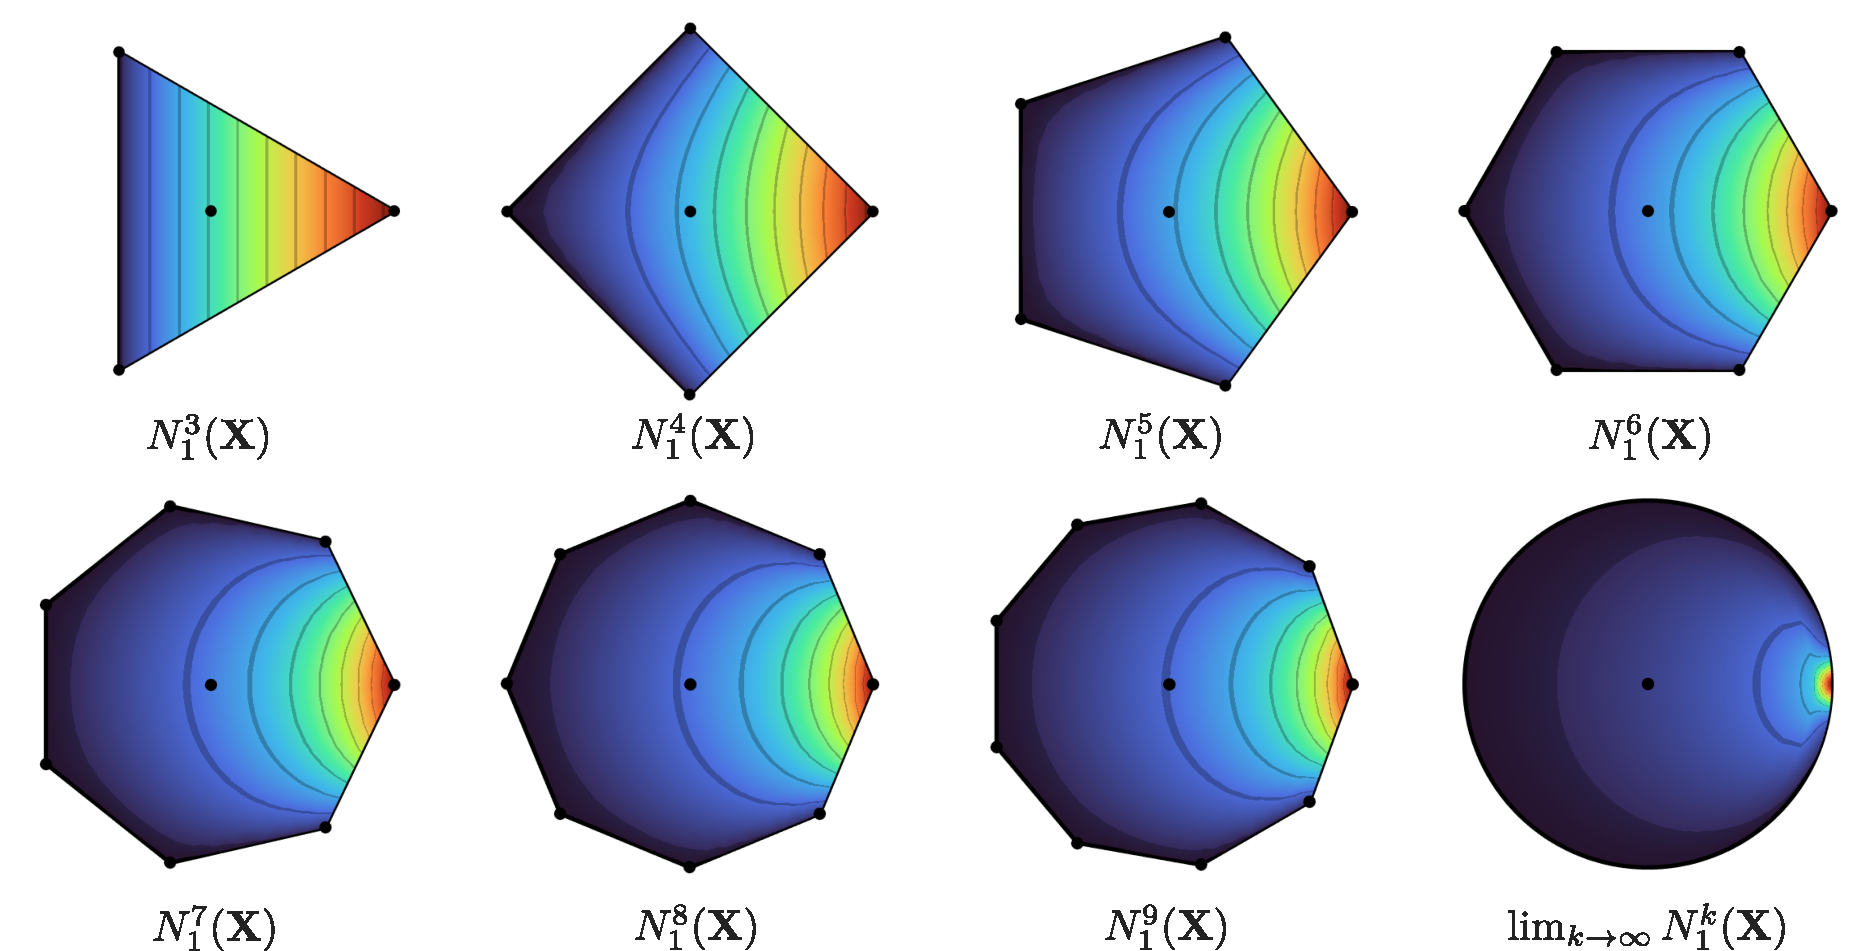
\includegraphics[width=\textwidth]{./pdf/thesis-figure-3-wachpress.pdf}
\caption{Wachspress shape functions related to the first nodal coordinate for an increasing polygonal degree $k$. The colormap depicts the intensity of the shape function $N_1^k$ with \protect\colormapcaption{0}{.75cm}$\!\!\in [0,1]$.}
\label{fig:C3:wachpressExample}
\vspace{-3mm}
\end{figure}
%

%With a discretized domain in mind, we can collect all the nodal displacements $\xB^{e}$ into one vector, called the global displacement vector $\xB = \textrm{col}(\x^{1},\x^{2},...,\x^{n_e})$. Similarly, we have a global virtual displacement vector $\delta \x$. 
Finally, by substitution of the spatial interpolations of the displacement $\dB \approx \NB^e \xB^e$ and virtual displacements $\delta \dB \approx \NB^e\delta \xB^e$, we can reformulate the residual in \eqref{eq:C3:residual_scalar} as follows
%
\begin{align}
\vec{r}	& \approx \sum_{e=1}^{n_e} ({\delta \xB}^e)^\top \left[\int_{\mathcal{V}_e} \BB_e(\x^e)^\top \underline{\ten{S}}_e(\x^e) \; dV  - \int_{\mathcal{V}_e} \NB^{e} \fB_{\textrm{b}} \; dV  - \int_{\p \mathcal{V}_e} \NB^{e} \fB_{\textrm{t}} \; dS \right], \notag \\[0.5em]
& = {\delta \x}^\top \left[ \fB_{\textrm{int}}(\xB) - \fB_{\textrm{ext}} \right],
\end{align}
%
where $\x$ and $\delta \x$ are the global nodal displacement and the global nodal virtual displacement vectors, and $\BB_e$ and $\underline{\ten{S}}_e$ the elemental strain-displacement matrix and Piolla stress tensor, respectively. The derivation of these elemental matrices is found Appendix \ref{app:C3:straindisplacement} which follows the work of Kim et al. \cite{Kim2018}. Since the entries of the displacement variation ${\delta \x}$ are zero at nodes where displacement is prescribed (\ie, fixed DoFs), we may consider an alternative form, the residual force vector, in which the virtual displacements are omitted by only regarding the free DoFs:
%
\begin{equation}
\RB(\x) = \fB_{\textrm{int}}(\x) - \fB_{\textrm{ext}},
\label{eq:residual}
\end{equation}
%

The static equilibrium of the structure can be determined by setting $\RB(\x)$, as given in \eqref{eq:residual}, equal to the zero vector. To obtain this equilibrium state, the Newton-Raphson method can be utilized through iterative calculation of a linear system \cite{Gain2013Dec,Kim2018,Holzapfel2002}:
%
\begin{align}
\KB_T^{(k)} \Delta \x^{(k)} & = \RB^{(k)}, \notag \\[0.25em]
\x^{(k+1)} & = \x^{(k)} + \Delta \x^{(k)}, \notag
\end{align}
%
where the subscript $(k)$ denotes the iteration steps, while $\x^{(k)}$, $\RB^{(k)}$, and $\KB_T^{(k)}:=\tfrac{\p \RB}{\p \x}\big|_{\x = \x^{(k)}}$ represent the updated displacement vector, the residual force vector, and the tangent stiffness matrix, respectively. For further details on the derivation of the tangent stiffness based on the Yeoh elasticity model in \eqref{eq:C3:psi_model_yeoh}, the reader is referred to Renaud et al. \cite{Renaud2011}, whose approach is outlined in Appendix \ref{app:C3:yeohmodel}.

% \begin{example}[Hyper-elastic uniaxial tension]
% %Before continuing
% \end{example}